\documentclass[12pt]{article}

\usepackage{geometry}
\geometry{margin=1in}
\usepackage{graphicx}
\usepackage[english]{babel}
\usepackage{fancyhdr}
\pagestyle{fancy}
\fancyhf{}
\lhead{Spring 2021 --- PHYS 421 Lab 2}
\rhead{Helen (Yeu) Chen}
\setlength{\parindent}{0cm}
\usepackage{makecell}
\usepackage{amsfonts}
\usepackage{longtable}
\usepackage{amsmath}
\usepackage{amssymb}
\usepackage{amsthm}
\usepackage{float}
\usepackage{caption}
\usepackage[outercaption]{sidecap}
\usepackage{multirow}
\graphicspath{ {./images/} }
\captionsetup[figure]{font=small,labelfont=small}


\fancyfoot[C]{\thepage}

\begin{document}
\textbf{X-Ray Spectra and Moseley’s Law Experiment}
\bigskip

\textbf{1. \textit{Introduction}}
\smallskip

In this experiment, we analyzed the X ray emission spectra of various elements across a wide range of atomic number $Z$ to determine the screening constant in Moseley's law. Then, we further use the trend we observed for known Z samples to determine the Z values for six unknown samples.

When the sample is exposed under the gamma rays emitted from a radioactive source, electrons in the atomic orbitals were knocked out by photons in the incident gamma ray, causing electrons from higher level orbital to drop down to fill in the holes. As electrons making this downward transitions, photons were emitted at frequency correspond to the energy difference between two levels, hence forming a X ray spectrum. To record the X ray spectrum for each sample we used a XR-100CR semiconductor detector. The incoming X rays is associated with the channel number of the detector according to its energy approximately on a linear scale. Using the Amp-Tek MCA Software, a histogram is generated for each run of measurement with the x axis represents the channel number and the y axis represents the number of times the X-ray with that specific energy is recorded. Then, by carefully identifying the X ray emitted by the sample from the background, the peak location (in terms of channel number) is plotted against Z for all the known sample, and we see all the spectral lines ($K_{\alpha}, K_{\beta}, L_{\alpha}, L_{\beta}$...etc) follow the same relationship (with a different constant C since $\text{channel number} \propto E \propto \frac{1}{\lambda}$) as the Moseley's law:
$$\frac{1}{\lambda} = C(Z- \sigma)^2$$
The screening constant $\sigma$ for each line can be obtained from fitting the known Z data. With this relation in hand, we then identified six unknown sample to be Cr, Ni, Ge, Mo, In, and W. To further confirm our identification results, a calibration function from channel number to energy is made from the known sample. We then used such function to convert the peaks we observed in the unknown samples to energy and verified that they indeed match the accepted transition energies values.
\bigskip

\textbf{2. \textit{Identifying the unknown samples}}
\smallskip

A major part in identifying the unknown samples is to determine the wether the peak observed is from the K lines or the L lines. To do this, we find patterns between the spectra of the known and unknown samples. The unknowns can be roughly be put into three categories. 

\textbf{I. Fe group:} unknown 1, 2, and 3

In this group, there are two strong peaks in gaussian shape around 1000 similar to Fe, which we know are $K_{\alpha1}$ and $K_{\beta}$ peaks. Below shows a comparison of unknown 1 (Left) and Fe (Right) spectra:


\begin{figure}[H]
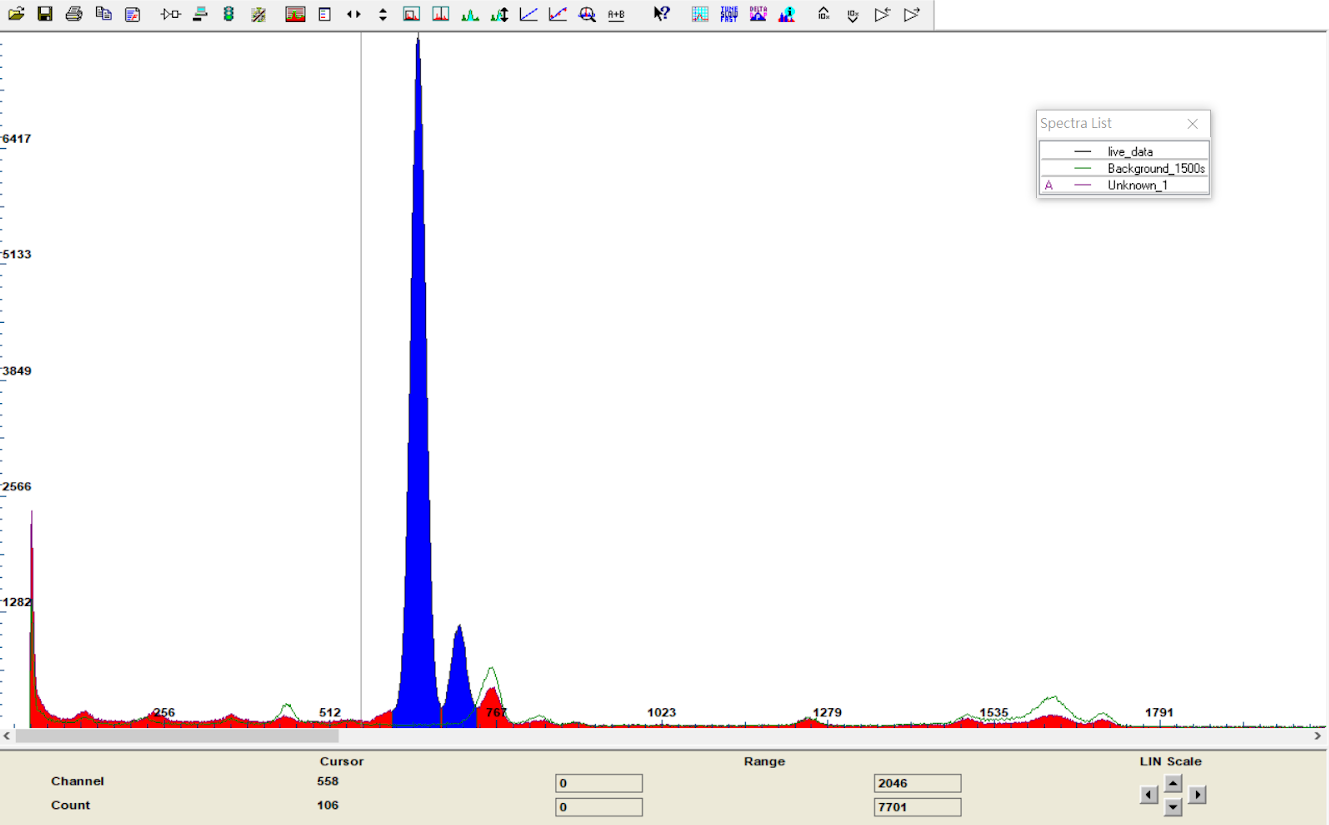
\includegraphics[width=8.5cm]{U1}
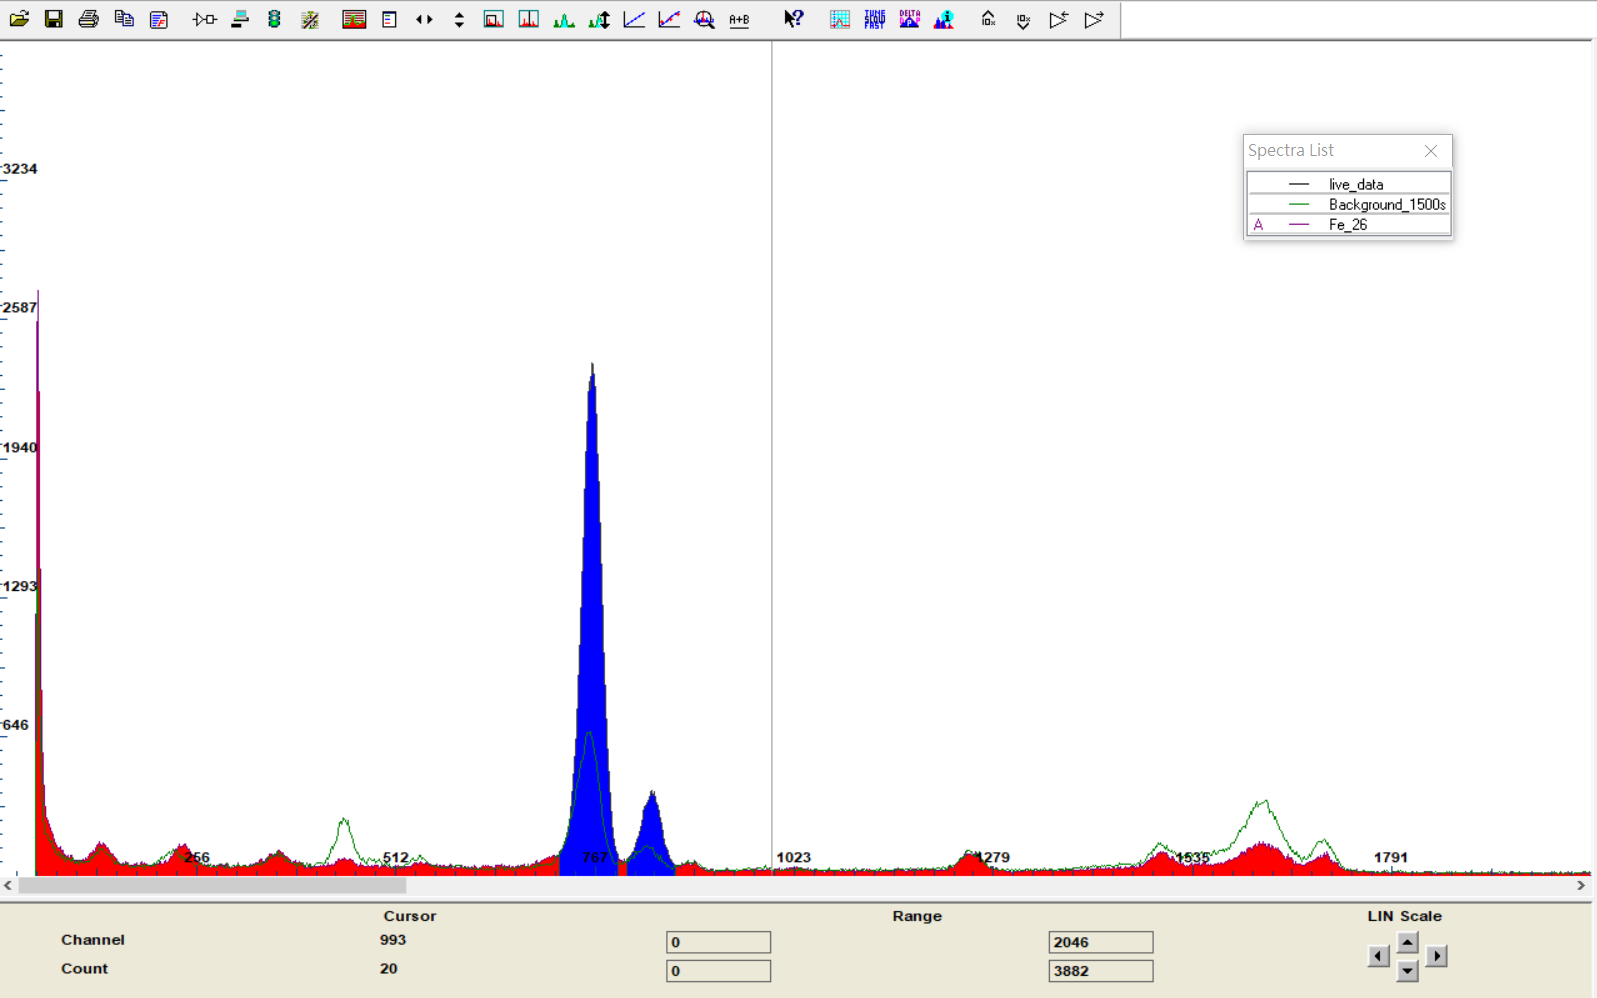
\includegraphics[width=8.5cm]{Fe_26}
\label{Fig. 1}
\caption{The X-ray spectrum histogram recored using the XR-100CR detector. The x axis represent the channel number, while the y axis represent the number of times the X ray with a specific channel energy is recorded. (Left) The spectrum of the sample unknown 1, with $K_{\alpha 1}$ and $K_{\beta}$ peaks highlighted in blue in the order from left to right. (Right) The Fe spectrum with $K_{\alpha 1}$ and $K_{\beta}$ peaks highlighted from left to right.}
\end{figure}
\smallskip

\textbf{II. Cd group:} unknown 4 and 5

In this group, there are three gaussian shaped peaks in the 2000 range with smaller intensity. Two are spaced closed to each other with the right one having stronger intensity. This pattern is seen in the spectrum of Cd, and from left to right, the peaks are $K_{\alpha2}, K_{\alpha1}, K_{\beta}$. Below shows a comparison of unknown 4 (Left) and Cd (Right) spectra (notice that the $L_{\alpha}$ is observed in Cd but not unknown 4 since its energy is too low to be seen in later):

\begin{figure}[H]
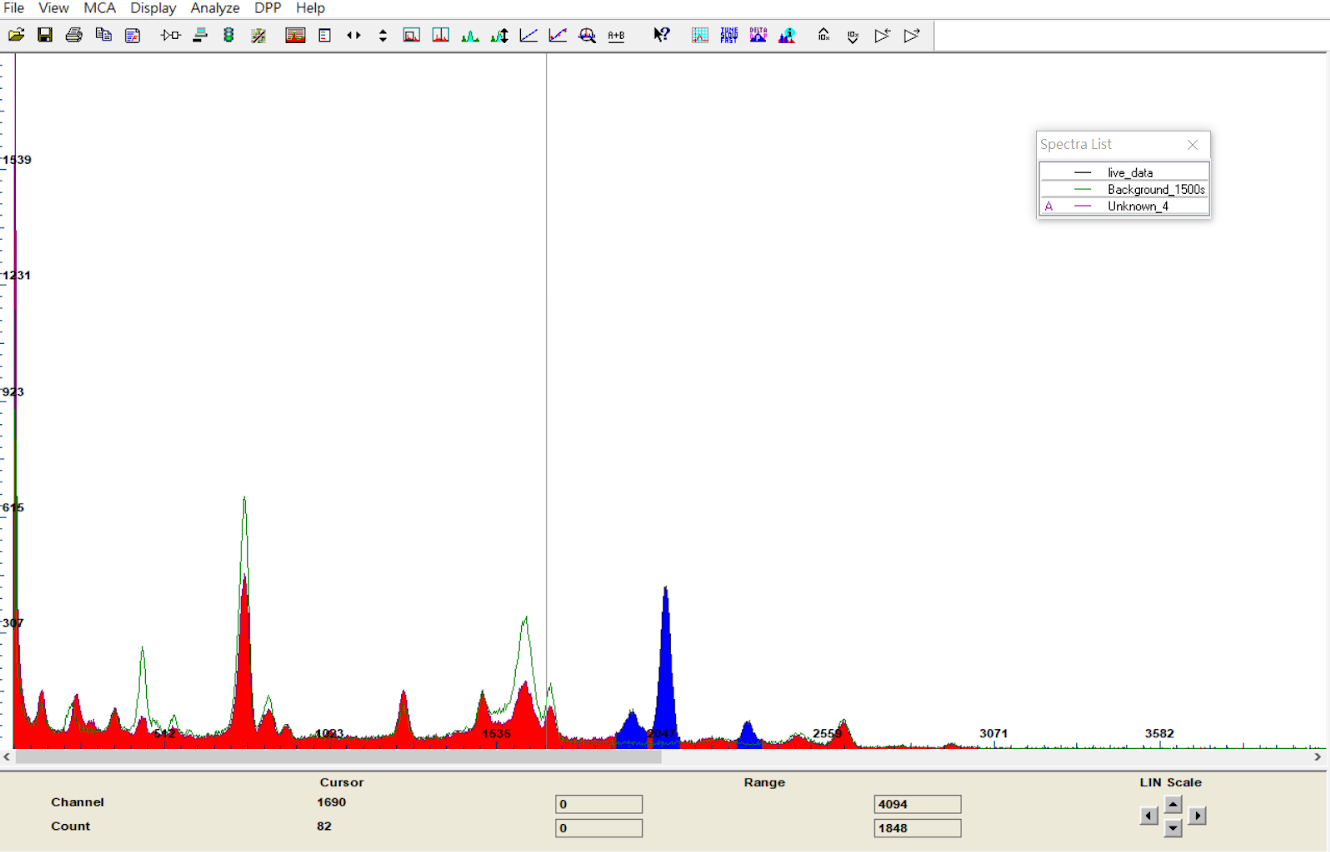
\includegraphics[width=8.5cm]{U4}
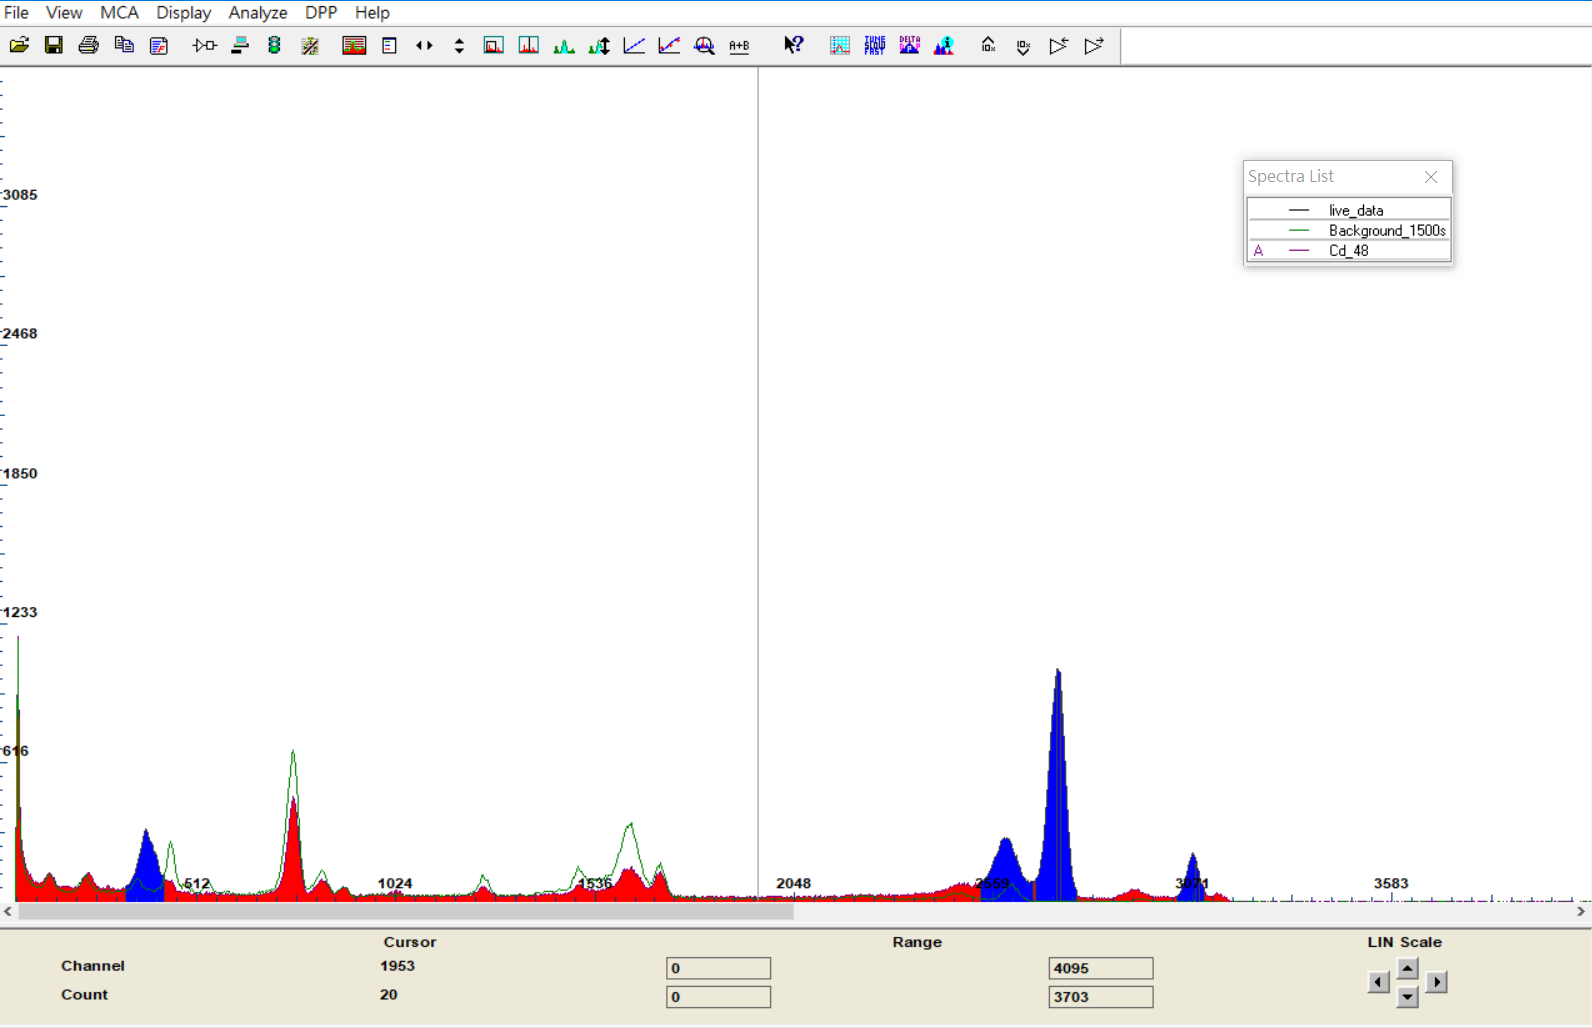
\includegraphics[width=8.5cm]{Cd_48}
\label{Fig. 2}
\caption{Similar spectrum collected from unknown 4 (Left) and Cd (Right) as which showed in Fig. 1. This time we are seeing $K_{\alpha2}, K_{\alpha1}, K_{\beta}$ transition, which are the left most three highlighted peaks, in the order from left to right. Notice there are an extra peak showing corresponding to the $L_{\alpha}$ transition for Cd, which we did not use in out comparison.}
\end{figure}
\smallskip

\textbf{III. Ta group:} unknown 6

In this group there are two not so symmetric peaks in the 1000 range with strong intensities. Notice their shape is very different from the K lines peaks above. A similar pattern is recorded for Ta, which are, from left to right, $L_{\alpha}$ and $L_{\beta}$ peak. Below shows a comparison of unknown 6 (Left) and Ta (Right) spectra:

\begin{figure}[H]
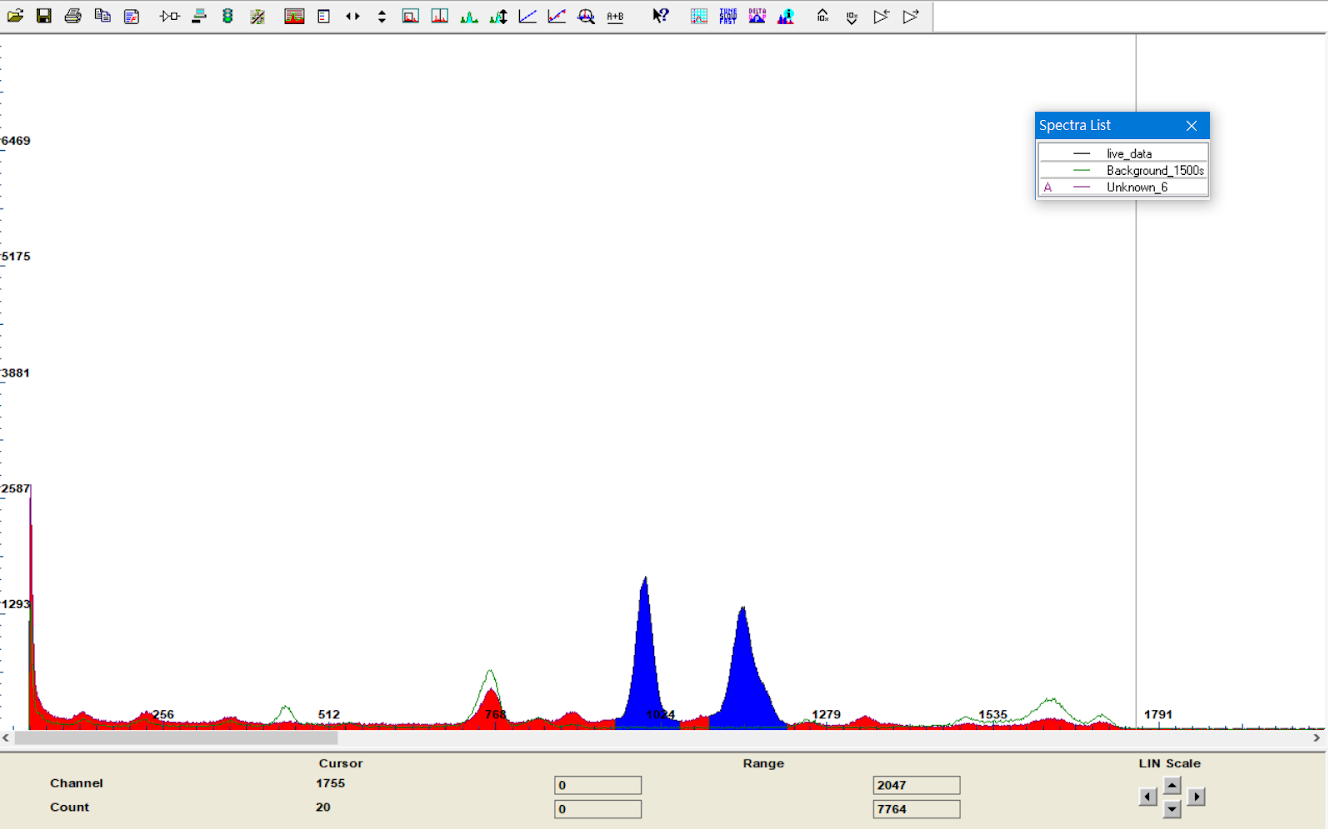
\includegraphics[width=8.5cm]{U6}
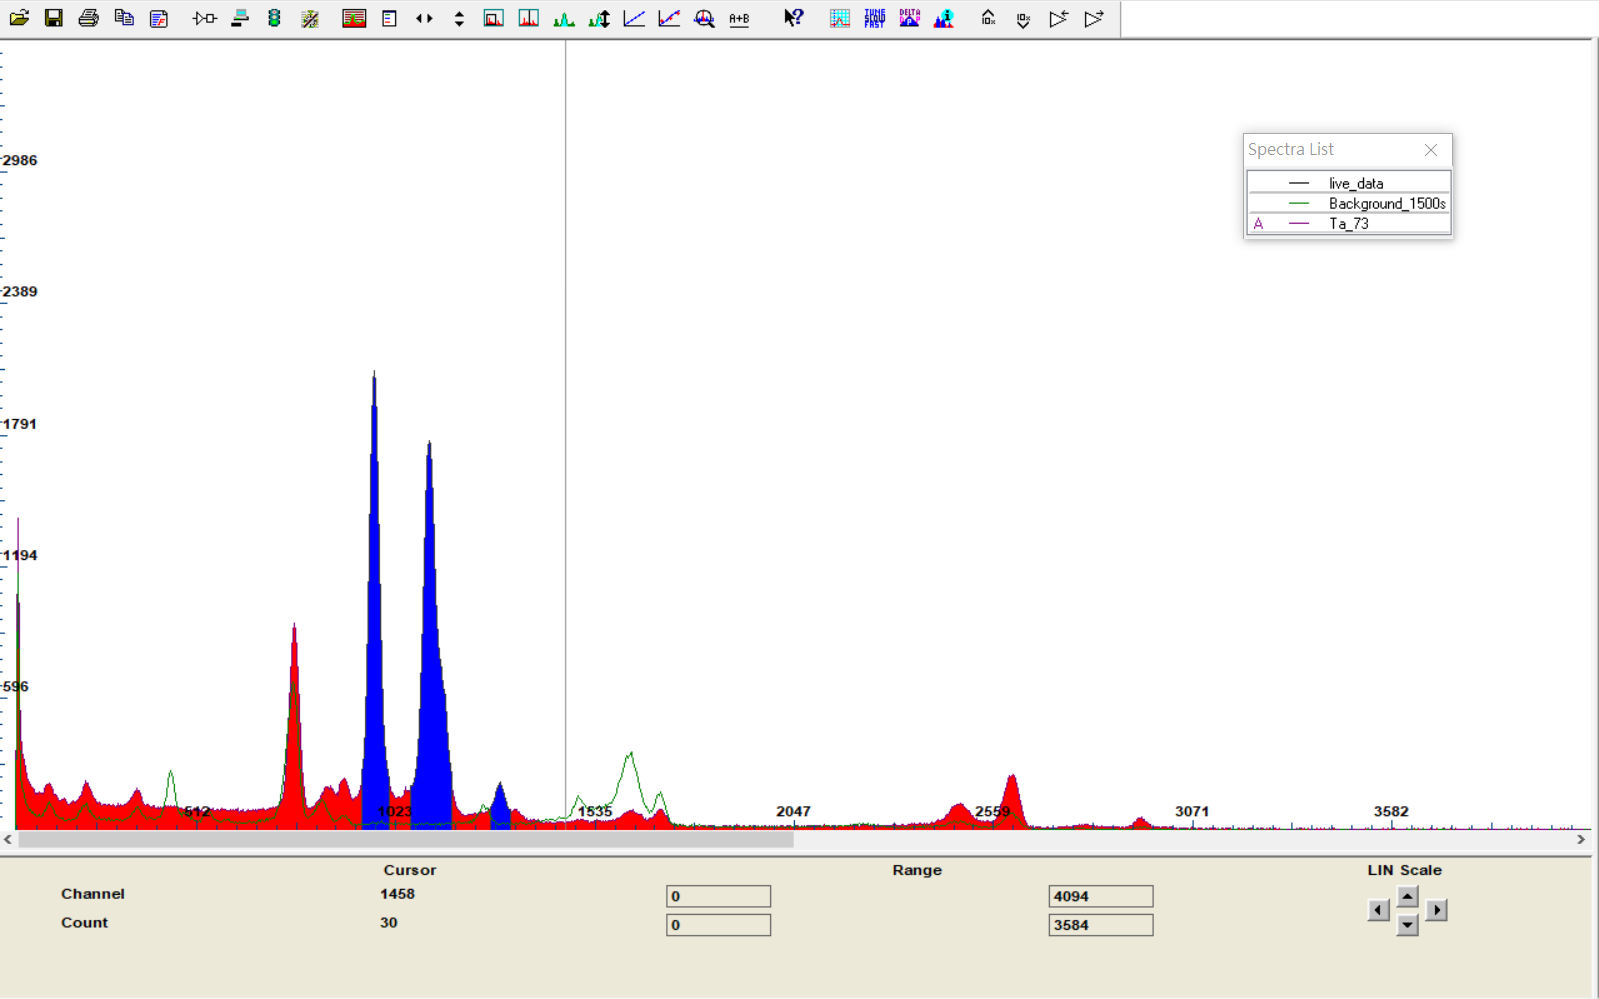
\includegraphics[width=8.5cm]{Ta_73}
\label{Fig.3}
\caption{Spectrum collected from from unknown 6 (Left) and Ta (Right). The two left most peaks in both pictures are $L_{\alpha}$ and $L_{\beta}$ peaks from left to right. For Ta, an extra $L_{\gamma}$ peak is showing which we did not used in our comparison.}
\end{figure}
\smallskip

Through this process, we have identified which shell transition each peak is belong to for all the unknown, we then can plot the peak locations with the fitted known samples (the known samples are: Cl, Ti, Cr, Fe, Ni, Cu, Zn, Ag, Cd, Sn, Gd, Ta, Au, and Pb), adjust the unknown's Z such that each peak lies on it's corresponding Moseley line (shown below).
We then found the Z values for unknown 1 to 6 are 24, 28, 32, 42, 49, and 74, which correspond to element Cr, Ni, Ge, Mo, In, and W.


\begin{SCfigure}[][h]
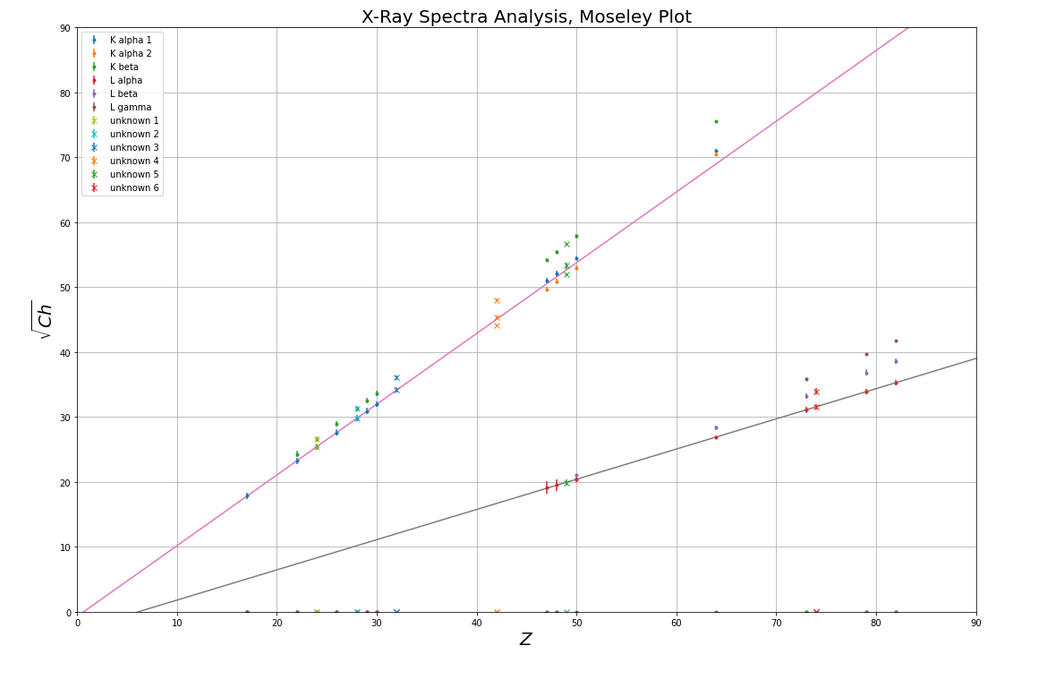
\includegraphics[width=10cm]{unknowns}
\label{Fig.4}
\caption{Moseley plot of Z vs square root of the channel number for both the knowns (solid dots) and the unknowns (crosses). The $K_\alpha$ and $L_\alpha$ transition for the knowns are fitted to a linear model, where the upper line with larger slope is the $K_\alpha$ fit line and the other is the $L_\alpha$ fit line. The unknowns' Z values are adjusted such that it's $K_\alpha$ and $L_\alpha$ data point lie on the corresponding fit lines.}
\end{SCfigure}
\bigskip

To further test our result, the calibration function we obtained from the known samples that convert channel number to energy is used. We calibrated peaks observed among the unknowns to energy and check these values with the accepted values using the "Amptek K and L Emission Line Lookup Chart", and found they agree with each other fairly well, and most of the accepted energies lie within the uncertainties of the measured values.

\begin{table}
\scriptsize
\begin{center}
\begin{tabular}{ |p{1cm}||p{1.9cm}|p{1.6cm}|p{1.9cm}|p{1.5cm}|p{1.9cm}|p{1.5cm}|p{1.9cm}|p{1.5cm}|  }
 \hline
 \multicolumn{9}{|c |}{Unknown samples measured vs. lookup energies in KeV} \\
 \hline
 element& measured $K_{\alpha 1}$&lookup $K_{\alpha 1}$&measured $K_{\beta}$&lookup $K_{\beta}$&measured $L_{\alpha}$&lookup $L_{\alpha}$&measured $L_{\beta}$&lookup $L_{\beta}$\\
 \hline
 Cr(24) & 5.425$\pm$0.013& 5.41&5.960$\pm$0.013&5.43& & & &\\
 Ni(28)&7.492$\pm$0.014&7.48&8.281$\pm$0.014&8.26& & & &\\
 Ge(32)&9.898$\pm$0.014&9.89&11.020$\pm$0.015&10.98& & & &\\
 Mo(42)&17.469$\pm$0.017&17.48&19.634$\pm$0.019&19.61& & & &\\
 In(49)&24.180$\pm$0.021&24.21&27.302$\pm$0.023&27.27& 3.285$\pm$0.013&3.29 & &\\ 
 W(74)&&&&&8.419$\pm$0.014 &8.40 &9.759$\pm$0.014 &9.67\\
 \hline
\end{tabular}
\end{center}
\label{Table 1}
\caption{A table showing the lookup energies for each elements from the "Amptek K and L Emission Line Lookup Chart" and the measured energy from the peak positions. As seen that most of the energies agree well within the uncertainties.}
\end{table}

\bigskip

\textbf{3. \textit{Aluminum}}
\smallskip

Aluminum has a $K_{\alpha1}$ energy of $1.49keV$ and a $K_{\beta1}$ energy of $1.55keV$. According to the calibration function we obtained from the known samples, they correspond to channel number $186$ and $193$ respectively, and in theory, we should see peaks there in the background. However, in the 120000s background below, we observed no peaks at these location (the vertical line is showing the position of channel 193). For our radioactive gamma ray source (Co 57) the $K_{\alpha1}$ energy is $6.93KeV$, which corresponds to a channel numbers of $823$. As seen from the plot below, we do observed peaks at channel number $831$ (highlighted in blue). Apart from the $K_\alpha$ energy we see from the Co, there is also the gamma ray from Co's radioactive decay, which is at about 14KeV. This energy corresponds to a channel number of about 1645, that is the second highest peak we see on the right in Fig.5. 

\begin{figure}[H]
\begin{center}
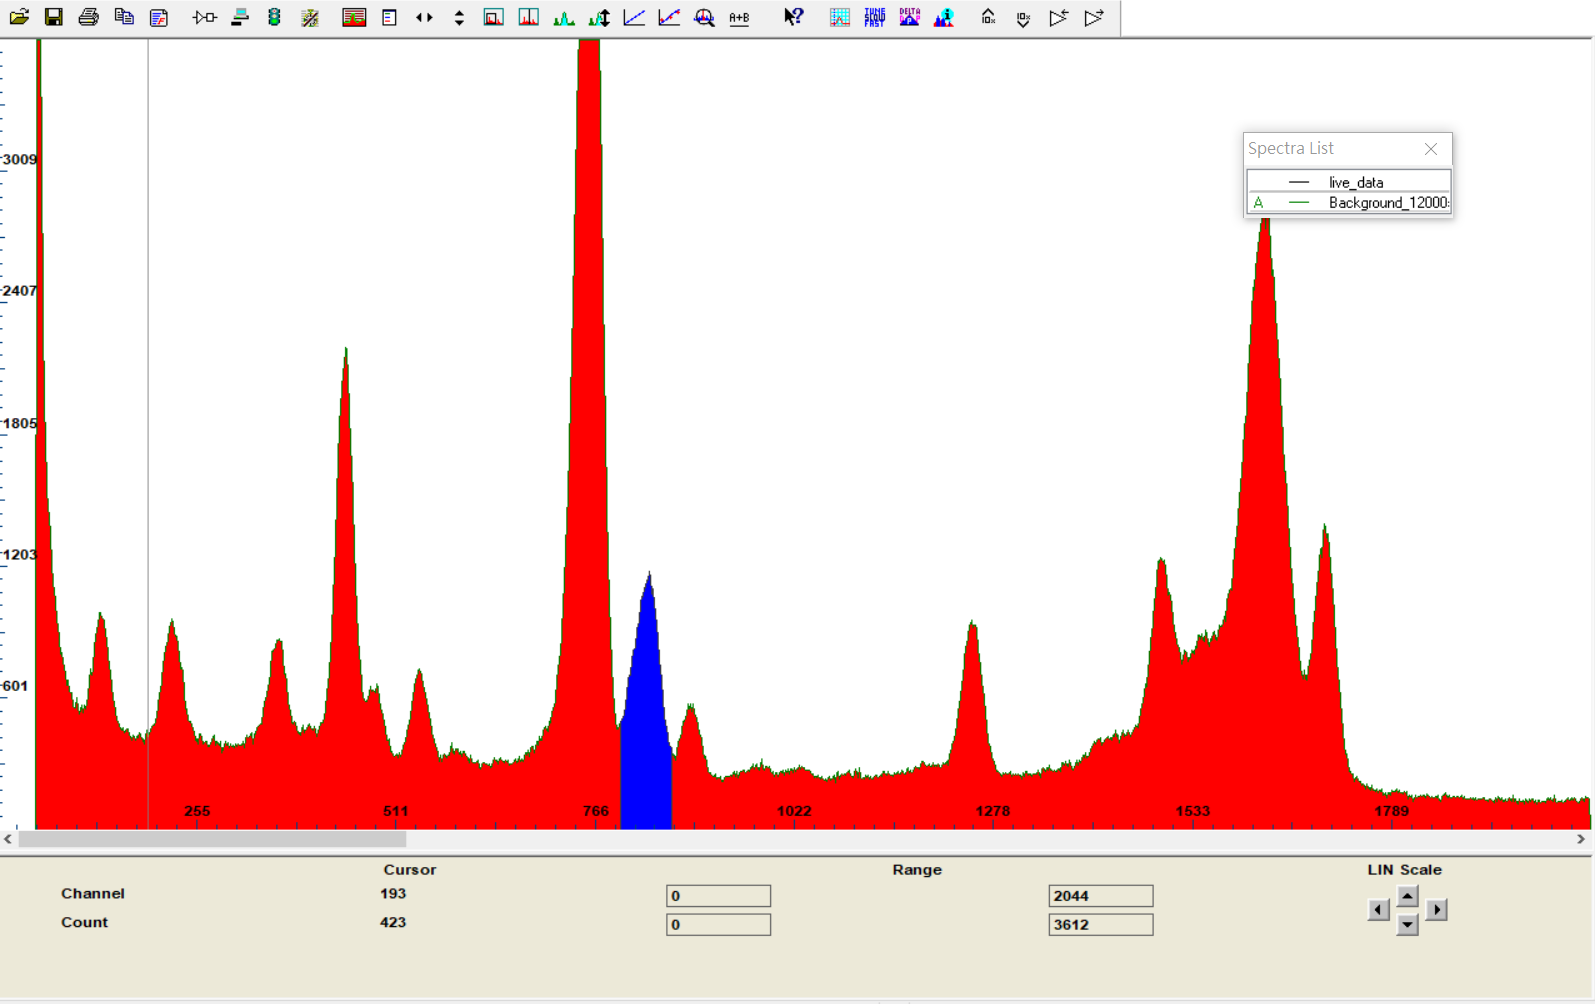
\includegraphics[width=12cm]{background}
\label{Fig. 5}
\caption{The background spectrum taken over a time period of 120000s. The highlighted peak correspond to the gamma ray from Co 57 $K_{\alpha 1}$ line at about channel number 831. The second peak from the right at about 1645 is also from Co. It correspond to the 14keV gamma ray emitted from Co's radioactive decay. The vertical line on the left at channel number 193 indicate the position where we should see the aluminum K peaks, which is not observed in the spectrum.}
\end{center}
\end{figure}

\end{document}